\documentclass[12pt]{letter}
\usepackage{amsmath,amsfonts,amsthm,amstext,amssymb,graphicx, multicol,fancyhdr,lastpage,fullpage,framed,fancybox,enumerate,tikz,color,mathrsfs, polynom}
\usepackage[margin=0.6in,headsep=3pt, headheight=15pt]{geometry}

% ----------------------------------------------------------
% Custom Definitions, Commands, Environments, etc.

% Sets of numbers
\def\R{\mathbb{R}} % The reals
\def\N{\mathbb{N}} % The naturals
\def\Z{\mathbb{Z}} % The integers
\def\Q{\mathbb{Q}} % The rationals

% Blank space
\newcommand{\blank}[1]{\underline{\hspace{#1}}} % Blank space

% Change font colors
\newcommand{\cyan}[1]{{\color{cyan}{#1}}} % Changes font to cyan
\newcommand{\red}[1]{{\color{red}{#1}}} % Changes font to red
\newcommand{\magenta}[1]{{\color{magenta}{#1}}} % Changes font to magenta
\newcommand{\orange}[1]{{\color{orange}{#1}}} % Changes font to orange
\newcommand{\yellow}[1]{{\color{yellow}{#1}}} % Changes font to yellow
\newcommand{\violet}[1]{{\color{violet}{#1}}} % Changes font to violet
\newcommand{\green}[1]{{\color{green}{#1}}} % Changes font to green
\newcommand{\blue}[1]{{\color{blue}{#1}}} % Changes font to blue
\newcommand{\white}[1]{{\color{white}{#1}}} % Changes font to white

% Fitted inclusion symbols
\newcommand{\fp}[1]{\left({#1}\right)} % Fitted parentheses around content
\newcommand{\fb}[1]{\left[{#1}\right]} % Fitted brackets
\newcommand{\set}[1]{\left\{{#1}\right\}} % Fitted braces (useful for sets)
\newcommand{\av}[1]{\left|{#1}\right|} % Fitted absolute value bars

% Augmented Matrix Environment
\newenvironment{amatrix}[1]{%
	\left[\begin{array}{@{}*{#1}{c}|c@{}}
	}{%
	\end{array}\right]
}

% Miscellaneous
\def\then{\Rightarrow}
\newcommand{\?}{\stackrel{?}{=}}

% To shortcut
\def\to{\rightarrow}



% Coordinate Plane (Four-Quadrant)
\def\coordplane {
	\begin{tikzpicture}		\draw[step=0.25cm,black,very thin,opacity=0.25] (-2.5cm, -2.5cm) grid (2.5cm, 2.5cm);
	\draw[<->,thick,black] (-2.5cm, 0) -- (2.5cm, 0) node[anchor=north west,pos=0.94,font=\scriptsize]{$x$};
	\draw[<->,thick,black] (0,-2.5cm) -- (0, 2.5cm) node[anchor=south east,font=\scriptsize,pos=0.94]{$y$};
	\end{tikzpicture}
}

% Coordinate Plane (One-Quadrant)
\def\onequad {
	\begin{tikzpicture}
	\draw[step=0.25cm, black, very thin, opacity=0.25] (0,0) grid (7.5cm,5cm);
	\draw[->, thick, black] (0,0) -- (7.5cm, 0) node[anchor=north west,font=\scriptsize,pos=0.94]{$x$};
	\draw[->, black, thick] (0,0) -- (0,5cm) node[anchor=south east,font=\scriptsize,pos=0.94]{$y$};
	\end{tikzpicture}
}

% Counters
\newcounter{exercise}

% Exercise environment (auto-numbered)
\newenvironment{exercise}[1][]{\begin{framed}\refstepcounter{exercise}\textbf{Exercise~\theexercise:} #1}{\end{framed}}

% Book exercise environment
\newenvironment{bex}[2][] {
	\begin{framed}
		\textbf{Book Exercise {#2}}#1
	\end{framed}
}
% ----------------------------------------------------------

\begin{document}
	\textbf{Assignment 2 Key \\ MAT 130}
	\begin{bex}{P.5.10}
		{
			
		}
	\end{bex} \vspace{-8pt}
	
	% My answer here
	$x + 5 \neq 0 \then x \neq -5$ \\
	Domain: $(-\infty, -5) \cup (-5, \infty)$
	
	% \vspace{}
	 \vfill % \newpage
	
	\begin{bex}{P.5.14}
		{
			
		}
	\end{bex} \vspace{-8pt}
	
	% My answer here
	$2x - 5 \geq 0 \then x \geq \dfrac52$ \\
	Domain: $\fb{\dfrac52, \infty}$
	
	% \vspace{}
	\vfill % \newpage
	
	\begin{bex}{P.5.28}
		{
			
		}
	\end{bex} \vspace{-32pt}
	
	% My answer here
	\begin{flalign*}
	\dfrac{4 + 3x - x^2}{2x^2 - 7x - 4} &= \dfrac{-\fp{x^2 - 3x - 4}}{2x^2 - 7x - 4} & \\
	&= -\dfrac{(x - 4)(x + 1)}{2x^2 - 8x + x - 4} \\
	&= -\dfrac{(x-4)(x+1)}{(2x + 1)(x-4)} & \\
	&= -\dfrac{x+1}{2x+1}
	\end{flalign*}
	
	% \vspace{}
	 \vfill % \newpage
	
	\begin{bex}{P.5.34}
		{
			
		}
	\end{bex} \vspace{-32pt}
	
	% My answer here
	\begin{flalign*}
	\dfrac{r}{r-1}\div \dfrac{r^2}{r^2 - 1} &= \dfrac{r}{r-1}\times \dfrac{r^2 - 1}{r^2} & \\
	&= \dfrac{1}{r-1}\times\dfrac{(r+1)(r-1)}{r} & \\
	&= \dfrac{r+1}{r}
	\end{flalign*}
	
	% \vspace{}
	\vfill % \newpage
	
	\begin{bex}{P.5.36}
		{
			
		}
	\end{bex} \vspace{-32pt}
	
	% My answer here
	\begin{flalign*}
	\dfrac{t^2 - t - 6}{t^2 + 6t + 9}\cdot\dfrac{t + 3}{t^2 - 4} &= \dfrac{(t-3)(t+2)}{(t+3)^2}\cdot\dfrac{t+3}{(t+2)(t-2)} & \\
	&= \dfrac{t+2}{(t+3)(t-2)}
	\end{flalign*}
	
	% \vspace{}
	 \vfill  \newpage
	
	\begin{bex}{P.5.42}
		{
			
		}
	\end{bex} \vspace{-8pt}
	
	% My answer here
	$\dfrac{x}{x+4}\fp{\dfrac{x-1}{x-1}} - \dfrac{6}{x-1}\fp{\dfrac{x+4}{x+4}} = \dfrac{x(x-1) - 6(x+4)}{(x-1)(x+4)}, x\neq -4, 1$
	
	
	% \vspace{}
	 \vfill % \newpage
	
	\begin{bex}{P.5.44}
		{
			
		}
	\end{bex} \vspace{-32pt}
	
	% My answer here
	\begin{flalign*}
	\dfrac{2}{x^2 - 9} + \dfrac{4}{x + 3} &= \dfrac{2}{(x+3)(x-3)} + \dfrac{4}{x+3}\fp{\dfrac{x-3}{x-3}} & \\
	&= \dfrac{2 + 4(x-3)}{(x+3)(x-3)}
	\end{flalign*}
	
	% \vspace{}
	\vfill % \newpage
	
	\begin{bex}{P.5.50}
		{
			
		}
	\end{bex} \vspace{-32pt}
	
	% My answer here
	\begin{flalign*}
	\dfrac{x+5}{\fp{\dfrac{x}{5} - 5}} &= \dfrac{\dfrac{x+5}{1}}{\dfrac{x - 25}{5}} & \\
	&= \dfrac{x+5}{1}\cdot\dfrac{5}{x - 25} & \\
	&= \dfrac{5(x+5)}{x-25}
	\end{flalign*}
	
	% \vspace{}
	\vfill % \newpage
	
	\begin{bex}{P.5.73}
		{
			
		}
	\end{bex} \vspace{-8pt}
	
	% My answer here
	To find the probability, we need to find the ratio of the area of the smaller rectangle to the area of the smaller rectangle. Recall that the area of a rectangle is found using the formula $A = \ell w$.
	
	Small Rectangle: $A = x\fp{\dfrac{x}{2}} = \dfrac{x^2}{2}$ \\
	Large Rectangle: $A = (2x + 1)(x)$
	
	Probability: \begin{flalign*}
	P &= \dfrac{A_{\text{small rectangle}}}{A_{\text{large rectangle}}} & \\
	&= \dfrac{\dfrac{x^2}{2}}{x(2x+1)} & \\
	&= \dfrac{x^2}{2}\cdot \dfrac{1}{x(2x+1)} & \\
	&= \dfrac{x}{2(2x+1)}
	\end{flalign*}
	
	% \vspace{}
	\vfill \newpage
	
	\begin{bex}{P.6.12}
		{
			
		}
	\end{bex} \vspace{-8pt}
	
	% My answer here
	Any point satisfying these conditions lies in Quadrant I, since both coordinates are positive.
	
	% \vspace{}
	\vfill % \newpage
	
	\begin{bex}{P.6.14}
		{
			
		}
	\end{bex} \vspace{-8pt}
	
	% My answer here
	If $xy > 0$, then either $x > 0$ and $y > 0$ or $x < 0$ and $y < 0$, because the product of a positive number and a negative number is a negative number. With this in mind, any point satisfying these conditions lies either in Quadrant I or in Quadrant III.
	
	% \vspace{}
	\vfill % \newpage
	
	\begin{bex}{P.6.16}
		{
			
		}
	\end{bex} \vspace{-8pt}
	
	% My answer here
	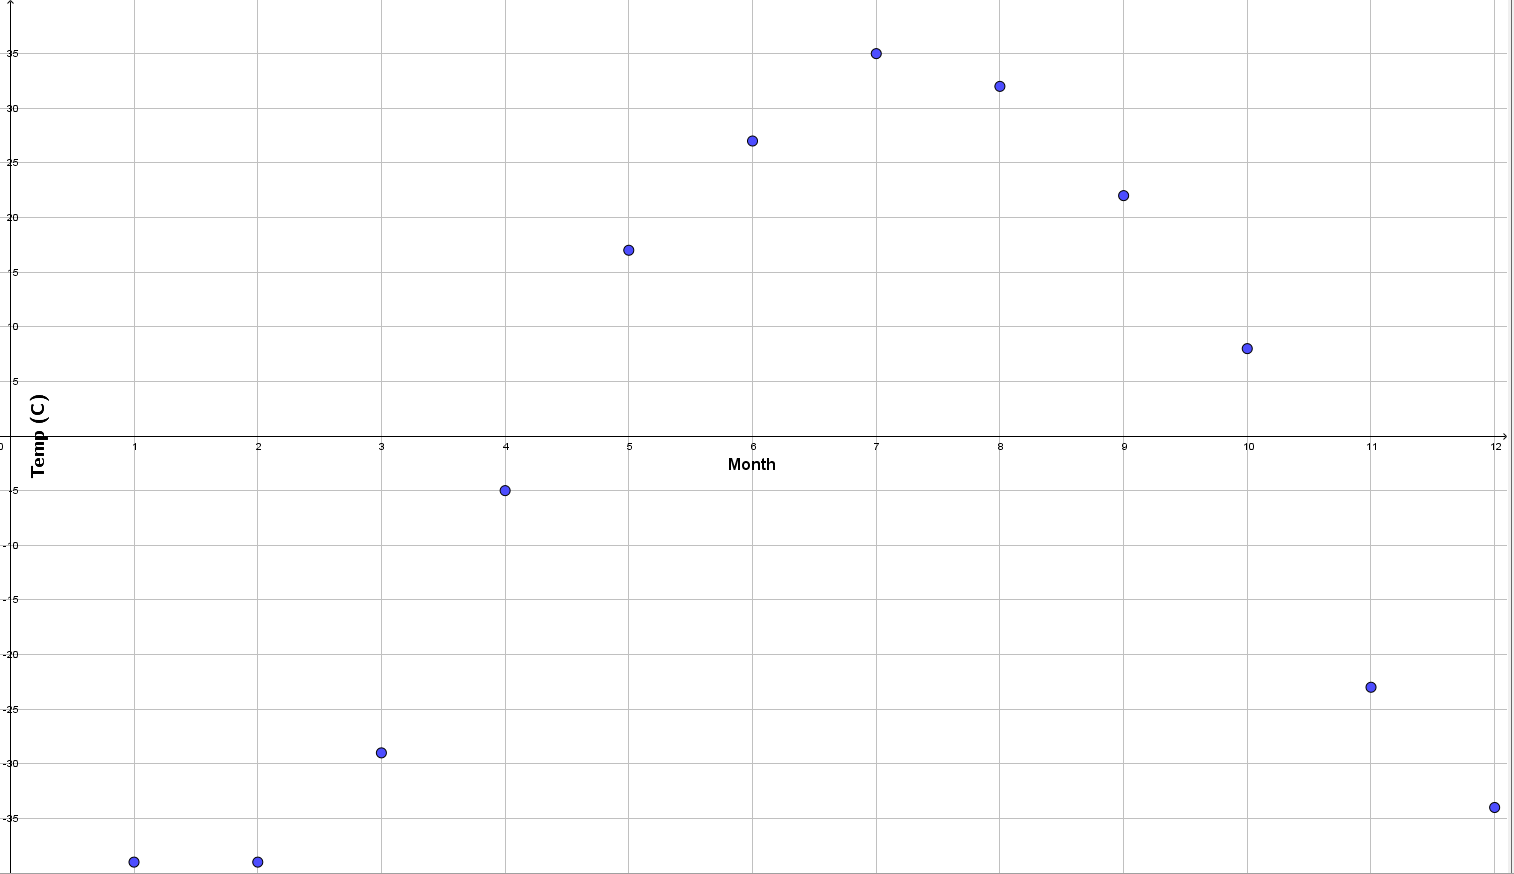
\includegraphics[width=6in]{P616.png}
	
	% \vspace{}
	\vfill % \newpage
	
	\begin{bex}{P.6.24}
		{
			
		}
	\end{bex} \vspace{-8pt}
	
	% My answer here
	(a) The lengths are: $10$, $3$, and $\sqrt{(9 - (-1))^2 + (4 - 1)^2} = \sqrt{109}$
	
	(b) $10^2 + 3^2 \? \fp{\sqrt{109}}^2 \then 109 \? 109$ is true, so the Pythagorean Theorem is satisfied.
	
	% \vspace{}
	\vfill \newpage
	
	\begin{bex}{P.6.32}
		{
			
		}
	\end{bex} \vspace{-8pt}
	
	% My answer here
	(a) 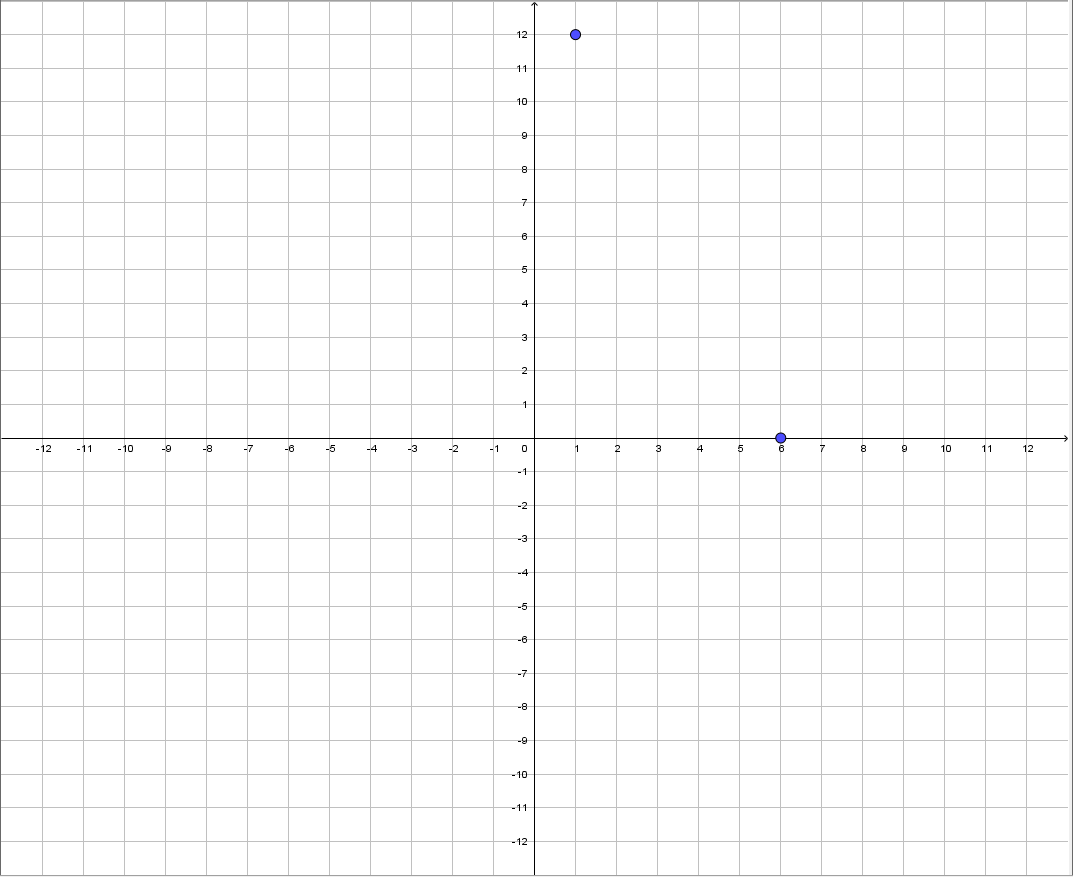
\includegraphics[width=2in]{P632a.png}
	
	(b) \begin{flalign*}
	D &= \sqrt{(x_2 - x_1)^2 + (y_2 - y_1)^2} & \\
	&= \sqrt{(6 - 1)^2 + (0 - 12)^2} & \\
	&= \sqrt{25 + 144} & \\
	&= \sqrt{169} & \\  &= 13
	\end{flalign*}
	(c) \begin{flalign*}
	M &= \fp{\dfrac{x_1 + x_2}{2}, \dfrac{y_1 + y_2}{2}} & \\
	&= \fp{\dfrac{1 + 6}{2}, \dfrac{12 + 0}{2}} & \\
	&= \fp{\dfrac72, 6}
	\end{flalign*}
	
	% \vspace{}
	\vfill % \newpage
	
	\begin{bex}{P.6.38}
		{
			
		}
	\end{bex} \vspace{-8pt}
	
	% My answer here
	We need to use the distance formula to determine the distance between $(12, 18)$ and $(50, 42)$. \begin{flalign*}
	D &= \sqrt{(50 - 12)^2 + (42 - 18)^2} & \\
	&= \sqrt{1444 + 576} & \\
	&= \sqrt{2020} & \\
	&\approx 44.94 \text{ yd}
	\end{flalign*}
	
	% \vspace{}
	\vfill %\newpage
	
	\begin{bex}{P.6.40}
		{
			
		}
	\end{bex} \vspace{-8pt}
	
	% My answer here
	To predict the revenue in 2014, we need to find the midpoint of the points $(2013, 1.17)$ and $(2015, 3.25)$. $M = (2014, 2.21)$ so we predict that revenue per share for Twitter, Inc. was \$2.21 in 2014.
	
	% \vspace{}
	\vfill \newpage
	
	\begin{bex}{P.6.44}
		{
			
		}
	\end{bex} \vspace{-8pt}
	
	% My answer here
	New Coordinates: $(-5, 2)$, $(-7, 0)$, $(-3, 0)$
	
	% \vspace{}
	\vfill % \newpage
	
	\begin{bex}{1.1.12}
		{
			
		}
	\end{bex} \vspace{-8pt}
	
	% My answer here
	(a) \vspace{-30pt} \begin{flalign*}
	3 &\? \av{2 - 1} + 2 & \\
	3 &\? 1 + 2 & \\
	(3, 2) & \text{ is a solution.}
	\end{flalign*}
	(b) \vspace{-30pt} \begin{flalign*}
	0 &\? \av{-1 - 1} + 2 & \\
	0 &\? 2 + 2 & \\
	(-1, 0) & \text{ is not a solution.}
	\end{flalign*}
	
	% \vspace{}
	% \vfill % \newpage
	
	\begin{bex}{1.1.18}
		{
			
		}
	\end{bex} \vspace{-8pt}
	
	% My answer here
	\begin{tabular}{|c|c|c|c|c|c|} \hline
		$x$ & $-2$ & $-1$ & $0$ & $1$ & $2$ \\ \hline
		$y$ & $1$ & $4$ & $5$ & $4$ & $1$ \\ \hline
		$(x,y)$ & $(-2, 1)$ & $(-1, 4)$ & $(0, 5)$ & $(1, 4)$ & $(2, 1)$ \\ \hline
	\end{tabular}

	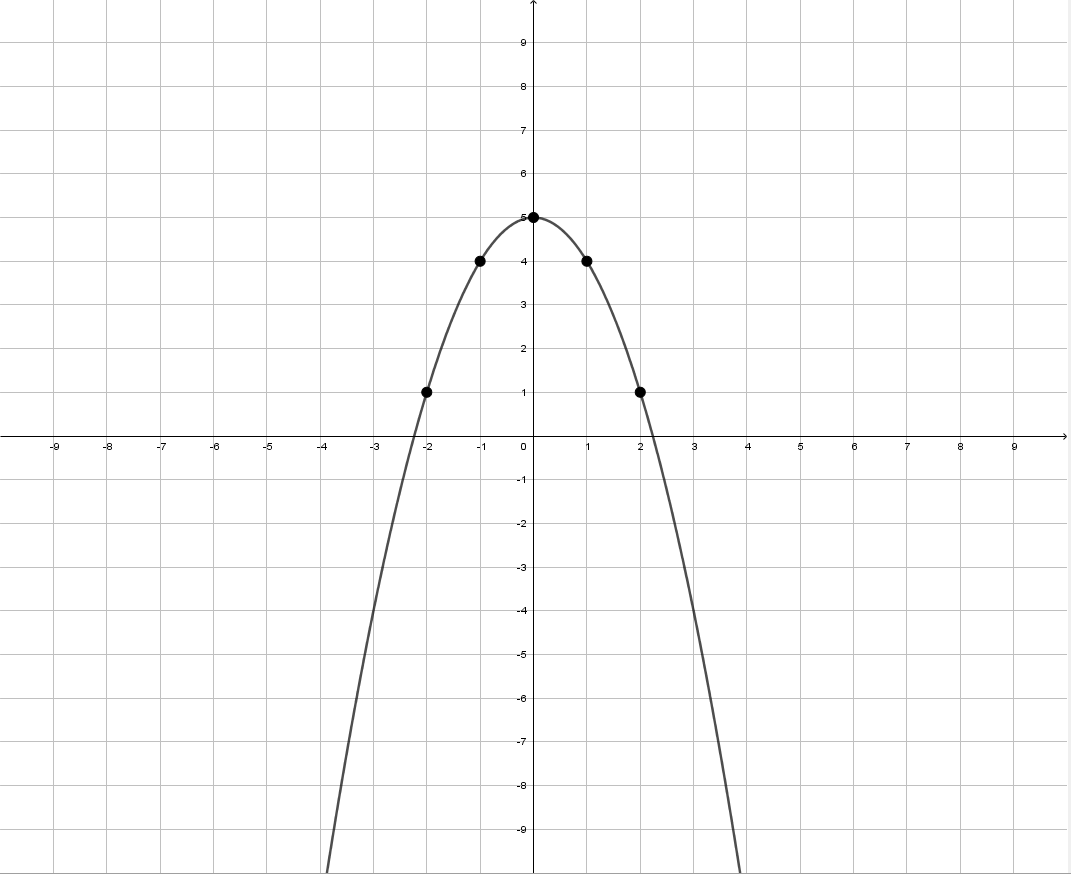
\includegraphics[width=3in]{1118.png}
	
	% \vspace{}
	\vfill % \newpage
	
	\begin{bex}{1.1.22}
		{
			
		}
	\end{bex} \vspace{-8pt}
	
	% My answer here
	$x$-intercept: $(4, 0)$ \\ $y$-intercepts: $(0, 2)$, $(0, -2)$
	
	% \vspace{}
	\vfill \newpage
	
	\begin{bex}{1.1.28}
		{
			
		}
	\end{bex} \vspace{-8pt}
	
	% My answer here
	\underline{Symmetry about $x$-axis:} \\
	$-y = x^4 - x^2 + 3 \then y = -x^4 + x^2 - 3$ \\
	Not the same, so the graph is not symmetric about the $x$-axis.
	
	\underline{Symmetry about $y$axis:} \\
	$y = \fp{-x}^4 - \fp{-x}^2 + 3 \then y = x^4 - x^2 + 3$ \\
	Same, so the graph is symmetric about the $y$-axis.
	
	\underline{Symmetry about origin:} \\
	$-y = \fp{-x}^4 + \fp{-x}^2 + 3 \then -y = x^4 - x^2 + 3$ \\
	Not the same, so the graph is not symmetric about the origin.
	% \vspace{}
	\vfill % \newpage
	
	\begin{bex}{1.1.32}
		{
			
		}
	\end{bex} \vspace{-8pt}
	
	% My answer here
	\underline{Symmetry about $x$-axis:} \\
	$x(-y) = 4 \then -xy = 4 \then xy=-4$ \\
	Not the same, so the graph is not symmetric about the $x$-axis.
	
	\underline{Symmetry about the $y$-axis:} \\
	$(-x)y = 4 \then -xy = 4$ \\
	Not the same, so the graph is not symmetric about the $y$-axis.
	
	\underline{Symmetry about the origin:} \\
	$(-x)(-y) = 4 \then xy = 4$ \\
	Same, so the graph is symmetric about the origin.
	
	% \vspace{}
	\vfill \newpage
	
	\begin{bex}{1.1.38}
		{
			
		}
	\end{bex} \vspace{-8pt}
	
	% My answer here
	\underline{Symmetry about $x$-axis:} \\
	$-y = 2x - 3 \then y = -2x + 3$ (not symmetric)
	
	\underline{Symmetry about $y$-axis:} \\
	$y = 2(-x) - 3 \then y = -2x - 3$ (not symmetric)
	
	\underline{Symmetry about origin:} \\
	$-y = 2(-x) - 3 \then y = 2x + 3$ (not symmetric)
	
	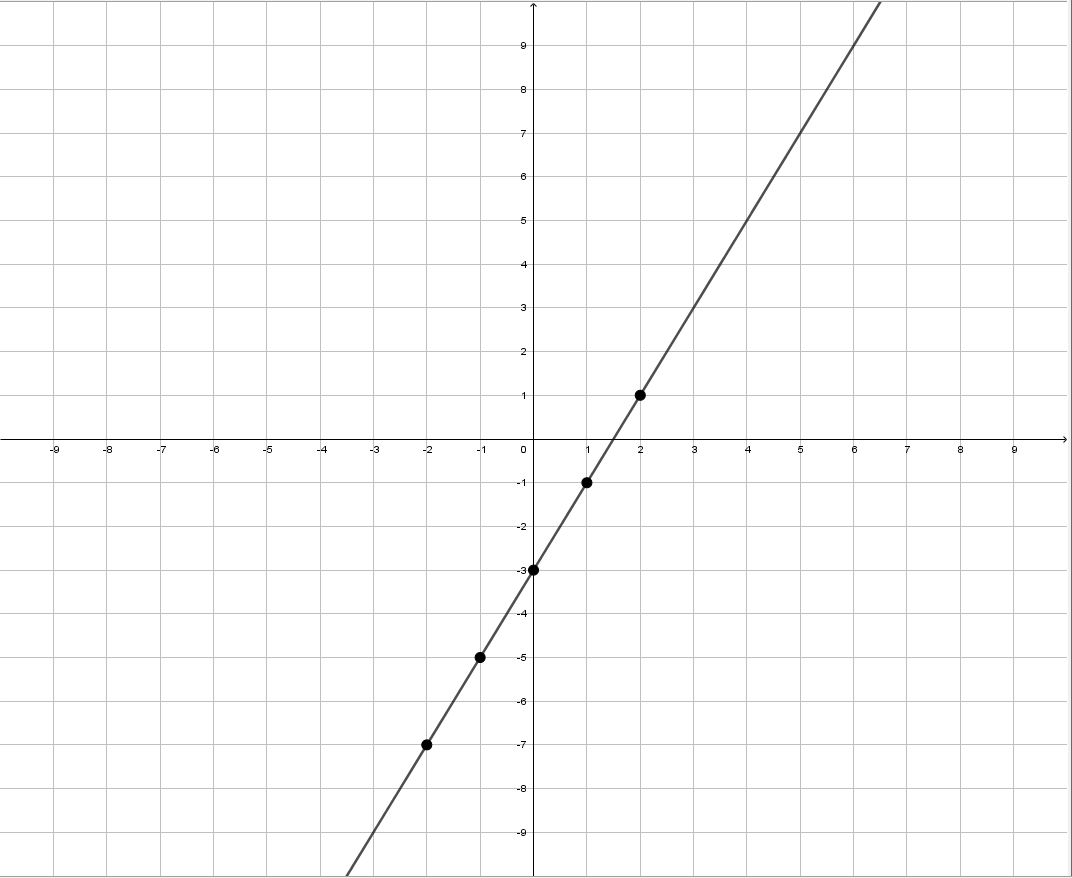
\includegraphics[width=2in]{1138.png}
	
	$x$-intercept: $\fp{\dfrac32, 0}$ \\ $y$-intercept: $(0, -3)$
	
	% \vspace{}
	\vfill % \newpage
	
	\begin{bex}{1.1.44}
		{
			
		}
	\end{bex} \vspace{-8pt}
	
	% My answer here
	\underline{Symmetry about $x$-axis:} \\
	$-y = \sqrt{1 - x} \then y = -\sqrt{1 - x}$ (not symmetric)
	
	\underline{Symmetry about $y$-axis:} \\
	$x = \sqrt{1 - (-x)} \then y = \sqrt{1 + x}$ (not symmetric)
	
	\underline{Symmetry about origin:} \\
	$-y = \sqrt{1 - (-x)} \then y = -\sqrt{1 + x}$ (not symmetric)
	
	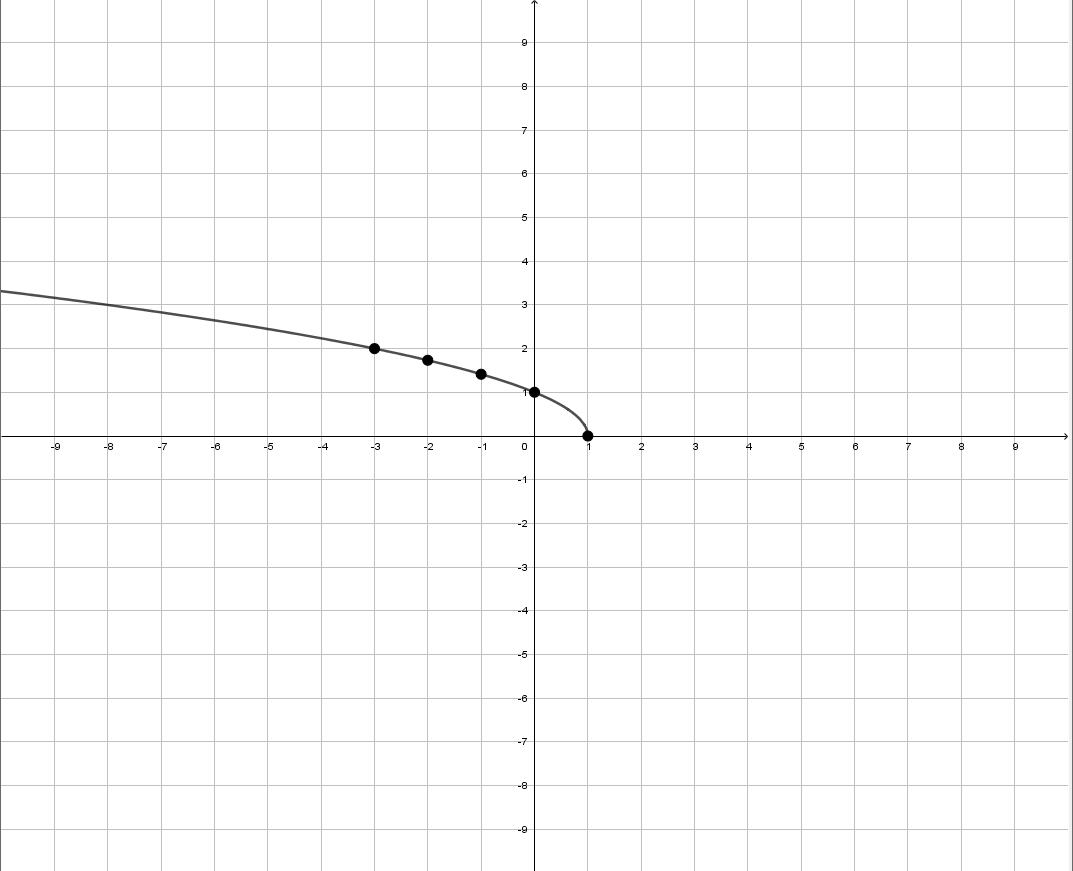
\includegraphics[width=2in]{1144.png}
	
	$x$-intercept: $(1, 0)$ \\ $y$-intercept: $(0,1)$
	
	% \vspace{}
	\vfill \newpage
	
	\begin{bex}{1.1.64}
		{
			
		}
	\end{bex} \vspace{-8pt}
	
	% My answer here
	In order to write the standard form equation for a circle, we need to know its center (already known) and its radius. Given the center and a point on the circle, we can find the radius using the Distance Formula: \begin{flalign*}
	D &= \sqrt{(1 - (-2))^2 + (-10 - (-6)^2)} & \\
	&= \sqrt{9 + 16} & \\
	&= 5
	\end{flalign*}
	
	Therefore, the standard form equation $\fp{(x-h)^2 + (y-k)^2 = r^2}$ is $(x - 1)^2 + (y + 10)^2 = 25$.
	
	% \vspace{}
	\vfill % \newpage
	
	\begin{bex}{1.1.70}
		{
			
		}
	\end{bex} \vspace{-8pt}
	
	% My answer here
	The circle given by this equation has a center at $(0, 1)$ and a radius of $1$.
	
	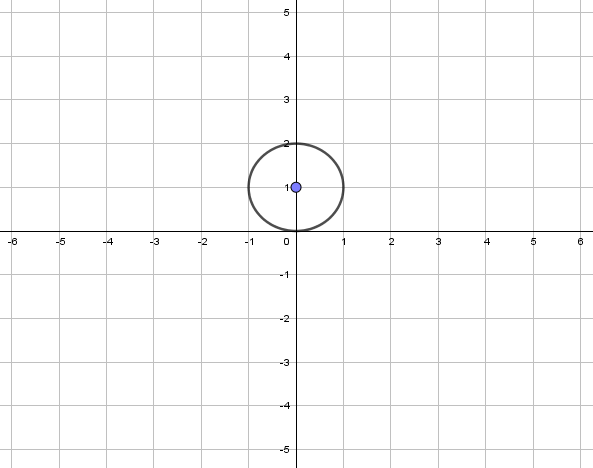
\includegraphics[width=3in]{1170.png}
	
	% \vspace{}
	\vfill % \newpage
	
	\begin{bex}{1.1.74}
		{
			
		}
	\end{bex} \vspace{-8pt}
	
	% My answer here
	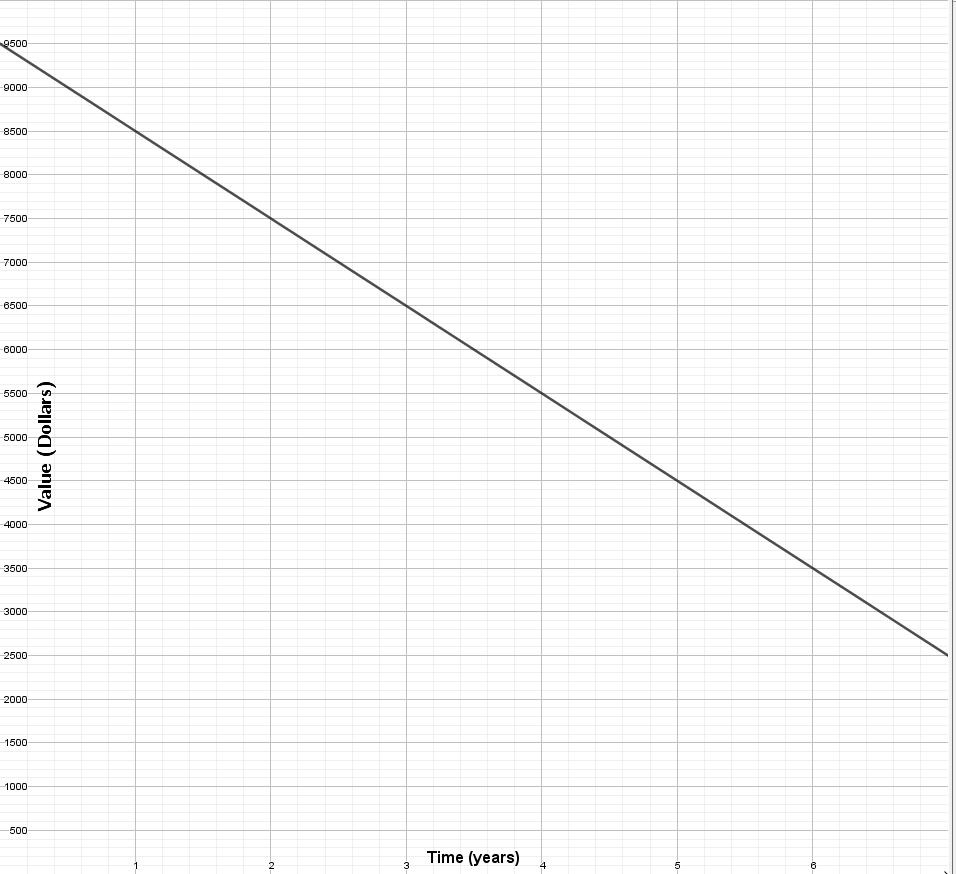
\includegraphics[width=3in]{1174.png}
	
	% \vspace{}
	\vfill \newpage
	
	\begin{bex}{1.2.24}
		{
			
		}
	\end{bex} \vspace{-32pt}
	
	% My answer here
	\begin{flalign*}
	9x - 10 &= 5x + 2(2x - 5) & \\
	9x - 10 &= 9x - 10 & \\
	0 &= 0
	\end{flalign*}
	Based on this result, we conclude that all real numbers are solutions to this equation.
	
	% \vspace{}
	% \vfill % \newpage
	
	\begin{bex}{1.2.28}
		{
			
		}
	\end{bex} \vspace{-32pt}
	
	% My answer here
	\begin{flalign*}
	\dfrac{2x}{5} + 5x &= \dfrac43 & \\
	6x + 75x &= 20 & \\
	81x &= 20 & \\
	x &= \dfrac{20}{81} & \\
	\dfrac{2\fp{\dfrac{20}{81}}}{5} + 5\fp{\dfrac{20}{81}} &\? \dfrac43 & \\
	\dfrac{\dfrac{40}{81}}{5} + \dfrac{100}{81} &\? \dfrac43 & \\
	\dfrac{40}{405} + \dfrac{500}{405} &\? \dfrac43 & \\
	\dfrac{540}{405} &= \dfrac{4}{3} & \checkmark
	\end{flalign*}
	
	% \vspace{}
	\vfill % \newpage
	
	\begin{bex}{1.2.34}
		{
			
		}
	\end{bex} \vspace{-32pt}
	
	% My answer here
	\begin{flalign*}
	\dfrac{15}{x} - 4 &= \dfrac{6}{x} + 3 & \\
	15 - 4x &= 6 + 3x & \\
	-7x &= -9 & \\
	x &= \dfrac97 & \\
	\dfrac{15}{\dfrac97} - 4 &\? \dfrac{6}{\dfrac97} + 3 & \\
	15\fp{\dfrac79} - 4 &\? 6\fp{\dfrac79} + 3 & \\
	\dfrac{105}{9} - 4 &\? \dfrac{42}{9} + 3 & \\
	105 - 36 &\? 42 + 27 & \\
	69 &= 69 & \checkmark
	\end{flalign*}
	
	% \vspace{}
	\vfill \newpage
	
	\begin{bex}{1.2.48}
		{
			
		}
	\end{bex} \vspace{-8pt}
	
	% My answer here
	\underline{Finding $x$-intercept:} \vspace{-8pt}
	\begin{flalign*}
	0 &= 5 - (6 - x) & \\
	0 &= -1 + x & \\
	x &= 1 & \\
	x\text{-intercept} &\text{ is $(0, 1)$.}
	\end{flalign*}
	\underline{Finding $y$-intercept:} \vspace{-8pt}
	\begin{flalign*}
	y &= 5 - (6 - 0) & \\
	y &= -1 & \\
	y\text{-intercept} & \text{is $(0, -1)$.}
	\end{flalign*}
	
	% \vspace{}
	\vfill % \newpage
	
	\begin{bex}{1.2.52}
		{
			
		}
	\end{bex} \vspace{-8pt}
	
	% My answer here
	\underline{Finding $x$-intercept:} \vspace{-8pt}
	\begin{flalign*}
	3(0) + 2.5x - 3.4 &= 0 & \\
	2.5x &= 3.4 & \\
	x &= \dfrac{25}{34} & \\
	x\text{-intercept} & \text{ is $\fp{\dfrac{25}{34}, 0}$.}
	\end{flalign*}
	\underline{Finding $y$-intercept:} \vspace{-8pt}
	\begin{flalign*}
	3y + 2.5(0) - 3.4 &= 0 & \\
	3y &= 3.4 & \\
	y &= \dfrac{30}{34} = \dfrac{15}{17} & \\
	y\text{-intercept} &\text{is $\fp{0, \dfrac{15}{17}}$}
	\end{flalign*}
	% \vspace{}
	\vfill % \newpage
	
	\begin{bex}{1.2.58}
		{
			
		}
	\end{bex} \vspace{-8pt}
	
	% My answer here
	Using a TI-84 Plus, I estimated a $y$-intercept of $-3$.
	\begin{flalign*}
	0 &= 10 + 2(x - 2) & \\
	0 &= 10 + 2x - 4 & \\
	-6 &= 2x & \\
	x &= -3
	\end{flalign*}
	
	% \vspace{}
	\vfill \newpage
	
	\begin{bex}{1.2.62}
		{
			
		}
	\end{bex} \vspace{-32pt}
	
	% My answer here
	\begin{flalign*}
	2.763 - 4.5(2.1x - 5.1432) &= 6.32x + 5 & \\
	2.763 - 9.45x + 23.1444 &= 6.32x + 5 & \\
	-9.45x + 25.9074 &= 6.32x + 5 & \\
	20.9074 &= 15.77x & \\
	x &\approx 1.326
	\end{flalign*}
	
	% \vspace{}
	% \vfill % \newpage
	
	\begin{bex}{1.2.70}
		{
			
		}
	\end{bex} \vspace{-8pt}
	
	% My answer here
	(a) It appears that the $y$-intercept is about $(0, 292)$.
	
	(b) $y = -2.60(0) + 291.7 \then y = 291.7$. The population of Buffalo, NY was about 291,700 in 2000.
	
	(c) \begin{flalign*}
	239 &= -2.60t + 291.7 & \\
	-52.7 &= -2.60t & \\
	t &\approx 20.27
	\end{flalign*} This means that the population of Buffalo, NY would reach 239,000 in 2020. If the population of the city continued dropping at a steady rate, the estimate would be accurate, but there are many factors that could cause a change in the trajectory. We have hindsight now; the population of Buffalo, NY in 2018 was about 256,304 so it seems doubtful that it will reach 239,000 in 2020.
	
	% \vspace{}
	% \vfill
\end{document}